\section{Halbleiter}

\subsection{Intrinsische Halbleiter (undotiert, Isolator)}

	\begin{minipage}{0.5\linewidth}
		Im intrinsischen Halbleiter gibt es immer gleich viele Elektronen und Löcher. 
		Diese werden durch die Bandlückenenergie $E_{Gap}$ getrennt. 
		Das obere Band ist das Leitungsband und das untere das Valenzband, da sich dort, 
		unterhalb der Fermi-Energie, die Valenzelektronen befinden. 
		Diese Elektronen-Loch-Paare können durch Photonen oder 
		durch Gitterschwingungen(Wärme) erzeugt werden, 
		daher leitet der Halbleiter auch besser bei hohen Temperaturen.
	\end{minipage}
	\begin{minipage}{0.5\linewidth}	
		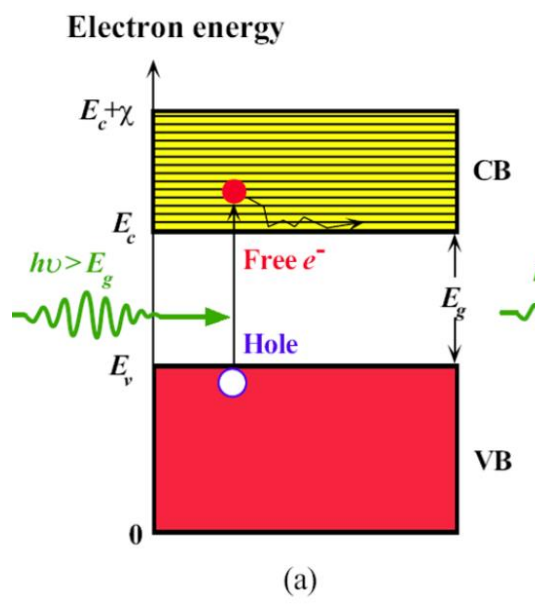
\includegraphics[width=0.85\linewidth]{Bilder/Intrinsischer_Halbleiter}
	\end{minipage}

	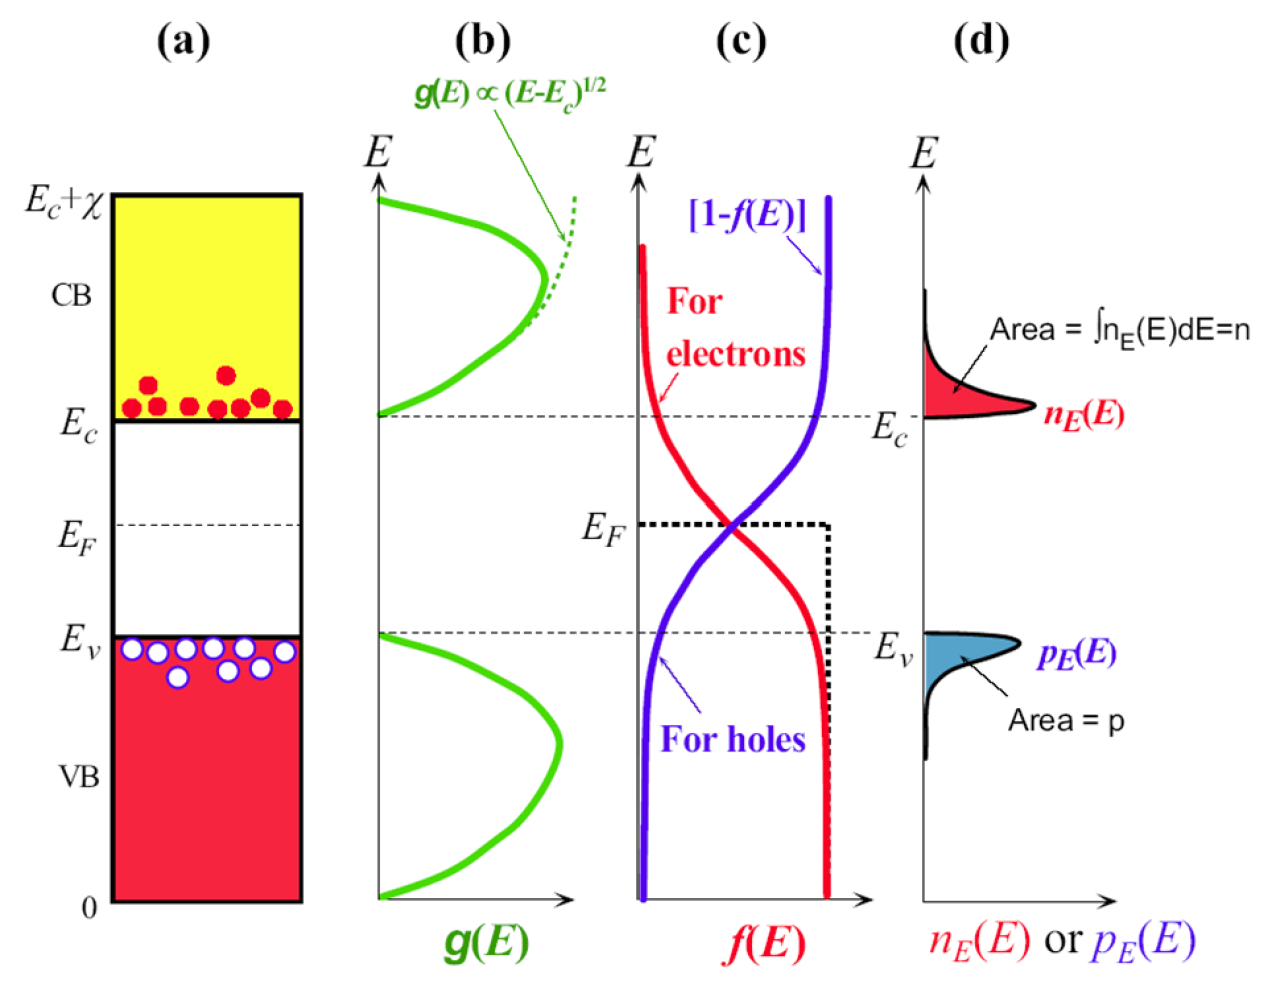
\includegraphics[width=0.8\linewidth]{Bilder/Intrinsischer_Halbleiter_Schema}	

	Fermi-Energie ist \textbf{in der Mitte} der Bandlücke ($E_F$)

	\begin{itemize}
		\item[(a)] Schematische Darstellung des Energiebandes im Ortsraum für einen Halbleiter
		\item[(b)] Zustandsdichte eines Halbleiters
		\item[(c)] Fermi-Dirac-Verteilung
		\item[(d)] Elektronen- bzw. Lochkonzentr. als Funktion $g(E) \cdot f(E) = n_E(E) \text{ resp. } p_E(E)$
	\end{itemize}

\subsection{Extrinsische Halbleiter (n-, p-dotiert)}
\begin{minipage}{0.49\linewidth}
	n-dotiert:

	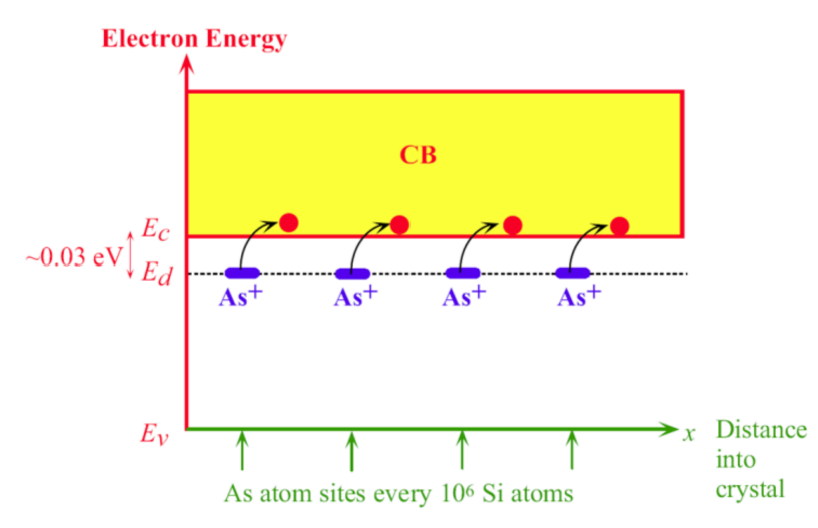
\includegraphics[width=\linewidth]{Bilder/Extrinsischer_Halbleiter-n}
\end{minipage}
\hfill
\begin{minipage}{0.49\linewidth}
	p-dotiert:

	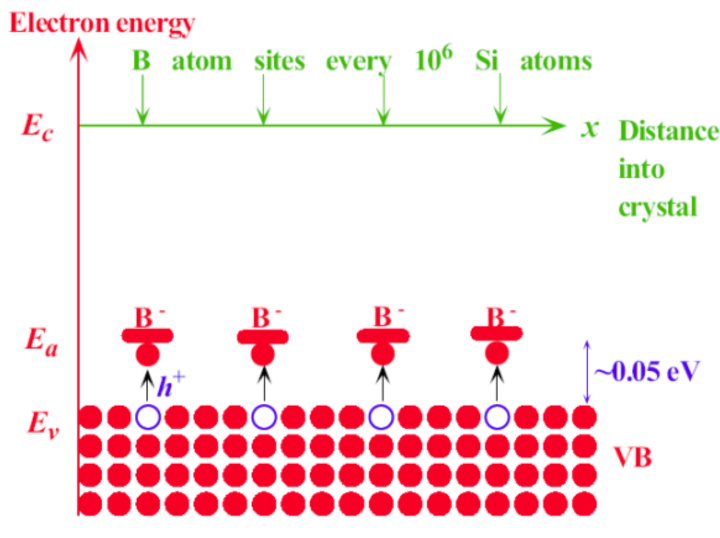
\includegraphics[width=0.9\linewidth]{Bilder/Extrinsischer_Halbleiter-p}
\end{minipage}


In extrinsischen Halbleiter ersetzt man im Si-Kristall einzelne Atome. 
\textbf{n-dotierte} Halbleiter entstehen durch Einsetzen von Atomen mit einem \textbf{überschüssigen} Elektron, 
\textbf{p-dotierte} Halbleiter durch Einsetzen von Atomen mit einem \textbf{fehlenden} Elektron. 
Die Konzentration von Dotierungsatomen ist sehr klein, nur etwa jedes $10^6$-te Atom wird ersetzt. 
Bei Raumtemperatur befinden sich die zusätzlichen Elektronen bereits im Leitungsband.

\subsection{Temperaturabhängigkeit}
\begin{minipage}{0.5\linewidth}
	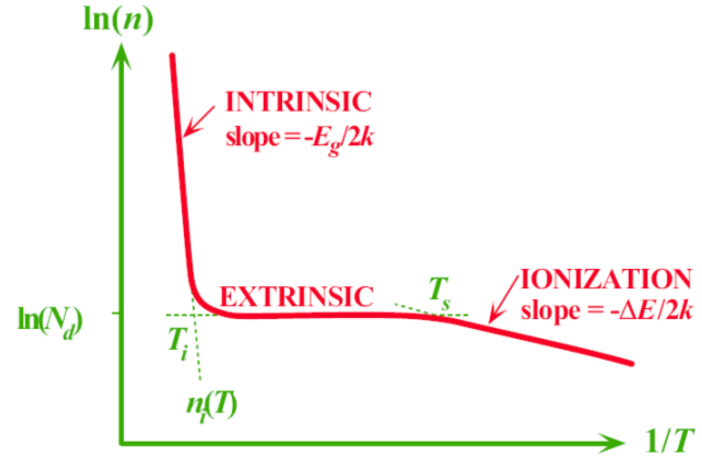
\includegraphics[width=0.9\linewidth]{Bilder/Temperaturabhängigkeit}
\end{minipage}
\begin{minipage}{0.5\linewidth}
	Wichtig für Halbleiteranwendungen ist der Bereich zwischen $T_s$ und $T_i$, 
	da dort die Ladungsträgerkonzentration konstant und temperaturunabhängig ist.
\end{minipage}

\subsection{Schottky-Diode ($\Phi_{metall} > \Phi_n$ oder $\Phi_{metall} < \Phi_p$)}
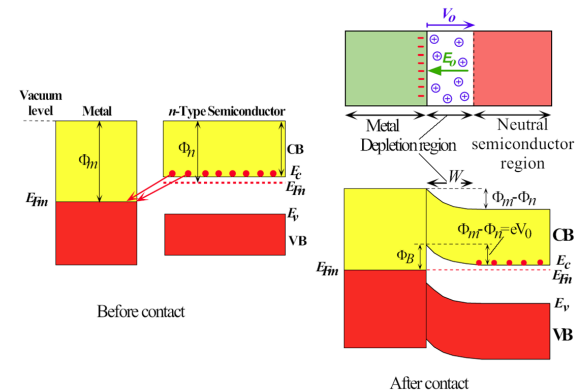
\includegraphics[width=0.9\linewidth]{Bilder/Schottky-Diode_1}

\begin{minipage}{0.5\linewidth}
	Durchlassrichtung:

	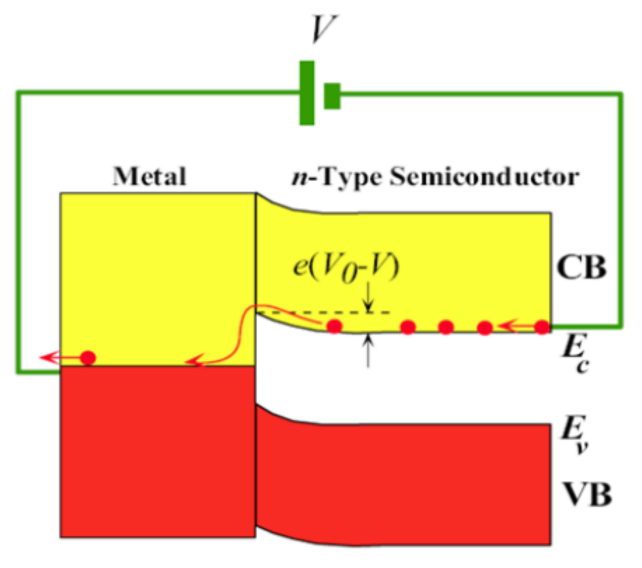
\includegraphics[width=0.9\linewidth]{Bilder/Schottky-Diode_2}	
\end{minipage}
\hfill
\begin{minipage}{0.5\linewidth}
	Sperrichtung:

	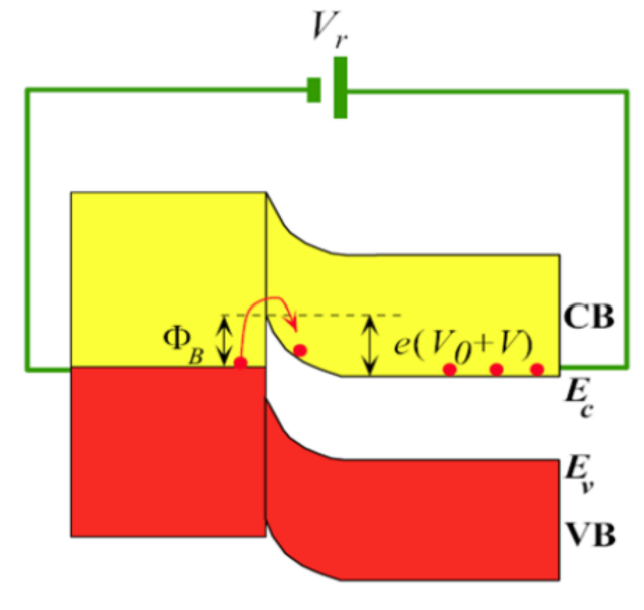
\includegraphics[width=0.9\linewidth]{Bilder/Schottky-Diode_3}		
\end{minipage}
Eine Schottky-Diode ist eine Verbindung von Metall und dotiertem Halbleiter. 
An der Kontaktfläche entsteht eine Verarmungszone. Da in dieser Zone keine Elektronen vorhanden sind, 
ist diese positiv geladen. Somit entsteht ein inneres elektrisches Feld. 
\begin{itemize}
	\item \textbf{Durchlass:} Potential des Halbleiters wird angehoben 
	\item[] $\to$ Elektronen überwinden Barriere
	\item \textbf{Sperrung:} Potential des Halbleiters wird abgesenkt 
	\item[] $\to$ kaum Elektronenfluss ($1\mu A$)
\end{itemize}

Sehr \textbf{schnelle Photodioden} werden mit Schottky-Dioden realisiert. 
Durch Anlegen einer Spannung in Sperrichtung wird die innere Spannung erhöht. 
Somit werden schneller die Elektronen-Loch-Paare getrennt und das Elektron kann schneller aus der Verarmungszone entweichen.

\subsection{Ohms'scher Kontakt ($\Phi_{metall} < \Phi_n$ oder $\Phi_{metall} > \Phi_p$)}
\begin{minipage}{0.49\linewidth}
	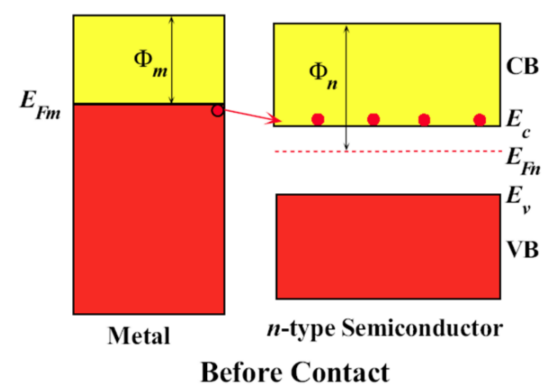
\includegraphics[width=0.9\linewidth]{Bilder/Ohmscher_Kontakt-before}
\end{minipage}
\hfill
\begin{minipage}{0.49\linewidth}
	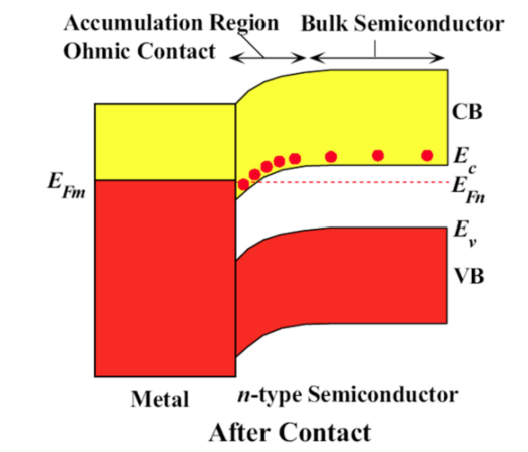
\includegraphics[width=0.9\linewidth]{Bilder/Ohmscher_Kontakt-after}
\end{minipage}

\begin{itemize}
	\item geringere Austrittsarbeit als Schottky-Diode
	\item \textbf{keine} Potentialbarriere
	\item Leitfähigkeit durch Halbleiterfähigkeit dominiert
	\item \textbf{nichtlineare} I-V-Kurve
\end{itemize}

% Ein Ohm'scher Kontakt ist auch eine Verbindung eines Metalls mit einem Halbleiter. 
% Der Unterschied zum Schottky-Kontakt ist, dass das Metall eine geringere Austrittsarbeit 
% als der Halbleiter hat. Es entsteht \textbf{keine} Potentialbarriere.

\subsection{Peltier-Effekt (bei Ohm'schen Kontakten)}
\begin{minipage}{0.5\linewidth}
	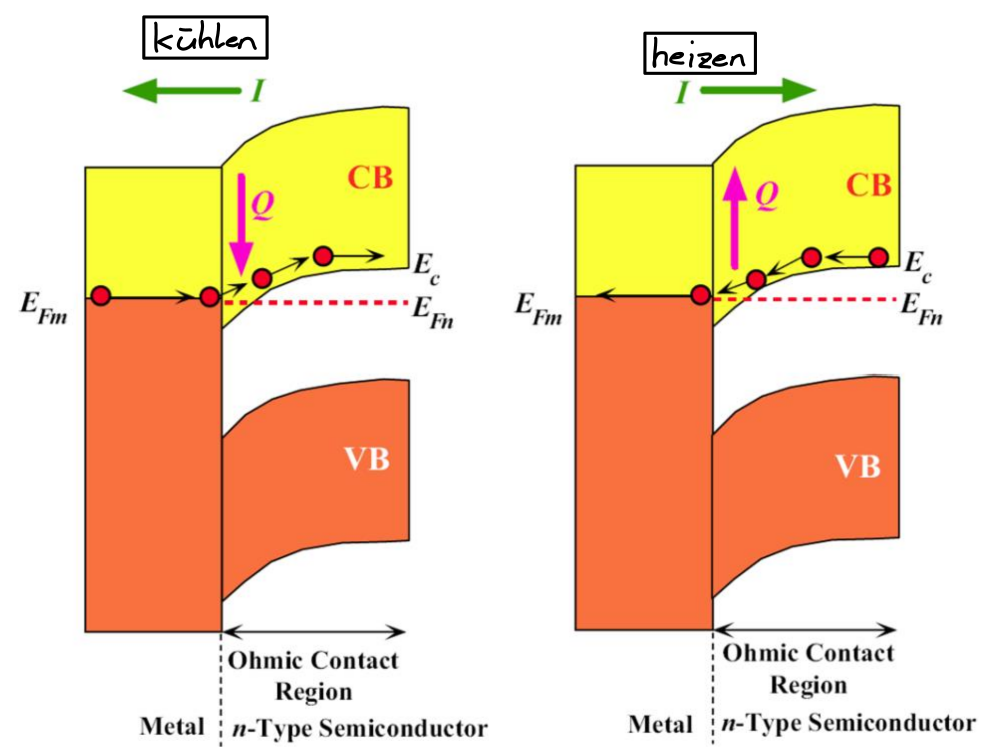
\includegraphics[width=0.99\linewidth]{Bilder/Peltier-Effekt}		
\end{minipage}
\begin{minipage}{0.5\linewidth}
	Wenn die Elektronen vom Metall zum Halbleiter fliessen, nehmen sie ein $\delta E$ an Energie auf, 
	um die Kontaktstelle(Akkumulationszone) zu überwinden.

	Diese Energie entnehmen sie der Umgebung(Phononen), welche sie abkühlt.

	Fliessen die Elektronen in die andere Richtung, wird die Umgebung erwärmt.
\end{minipage}

\begin{minipage}{0.4\linewidth}
	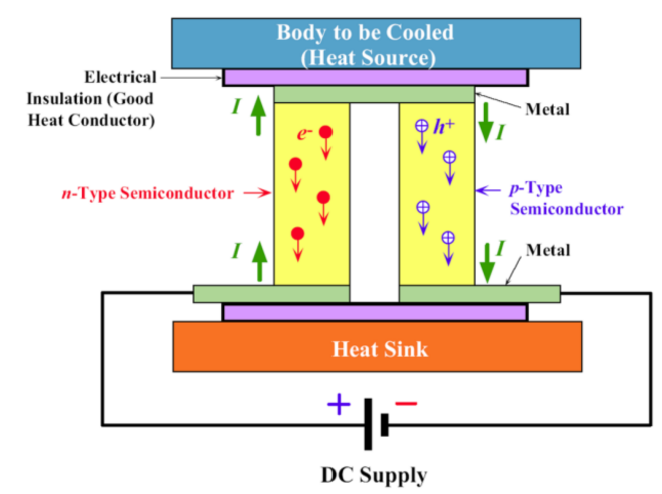
\includegraphics[width=0.99\linewidth]{Bilder/Peltier-1}
\end{minipage}
\hfill
\begin{minipage}{0.6\linewidth}
	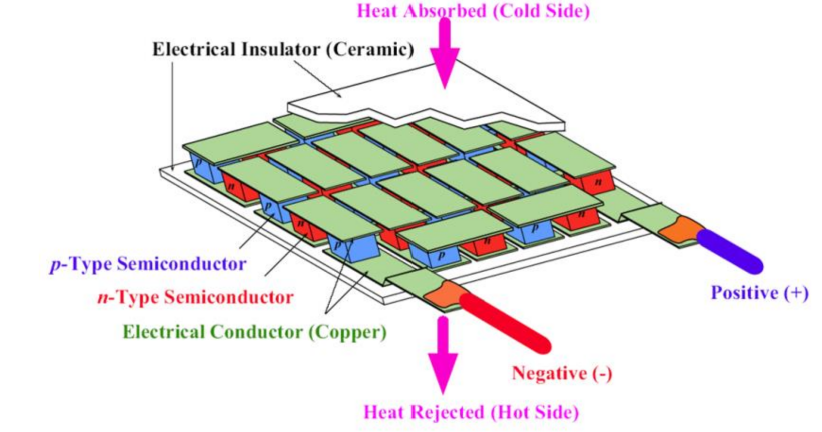
\includegraphics[width=0.99\linewidth]{Bilder/Peltier-2}
\end{minipage}